\documentclass{eh-homework}

\begin{document}
\usetikzlibrary{arrows.meta}
\section*{Assignment 3: Due March 16, 2025 (Sunday) at 11:59PM ET}

Answers must be submitted via Crowdmark using your personalized submission link (which will be sent to your email). Late submissions will not be accepted.

If you used Octave to assist you in solving a problem, also attach to the solution to that problem the script and commands you used and the corresponding outputs obtained.

A proper selection of questions from the ones below will be graded.

\begin{question}{1}
\textbf{(5.1, \#18)} The Bézier curve
\[
x(t) = 11t^3 - 18t^2 + 3t + 5
\]
\[
y(t) = t^3 + 1
\]
has control points \((5,1)\), \((6,1)\), and \((1,2)\). Find the fourth control point.

\bigskip

Notice that \((x(0), y(0)) = (5,1)\) and \((x(1), y(1)) = (1,2)\), so \((5,1), (1,2)\) are the first and last control points. Let us suppose that \((a,b)\) is the fourth control point, and it is ordered second.
\end{question}

\begin{question}{2}
Sketch a stencil for the following data, picking appropriate \(x_0\) and \(h\), that can be used to approximate \(f'(1)\). You do not need to derive the formula.

\[
\begin{array}{c|cccc}
x & -3 & -1.5 & 0 & 2 \\
\hline
f(x) & 3.11 & 3.05 & 3.4 & 3.7 \\
\end{array}
\]

\bigskip

We let \(x_0 = -3\), \(h = 1\). Then the stencil looks like this:
\begin{center}
    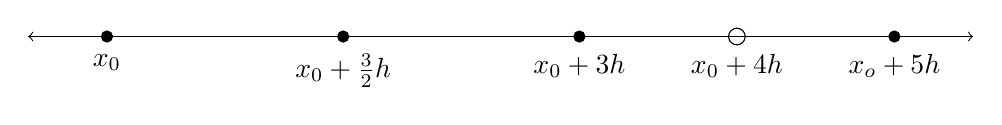
\begin{tikzpicture}
        \draw[<->] (-7, 0) -- (5, 0);
        \foreach \x\val in {-6/\(x_0\), -3/\(x_0 + \frac{3}{2}h\), 0/\(x_0 + 3h\), 4/\(x_o + 5h\)} {
            \draw[fill] (\x, 0) circle (2pt);
            \node[below] at (\x, -0.1) {\val};
        }
        \draw (2, 0) circle (3pt);
        \node[below] at (2, -0.1) {\(x_0 + 4h\)};
    \end{tikzpicture}
\end{center}
\end{question}

\begin{question}{3}
\textbf{(4.1, \#13c)} Derive an approximation formula for the second derivative \( f'' \) over the stencil:

\begin{center}
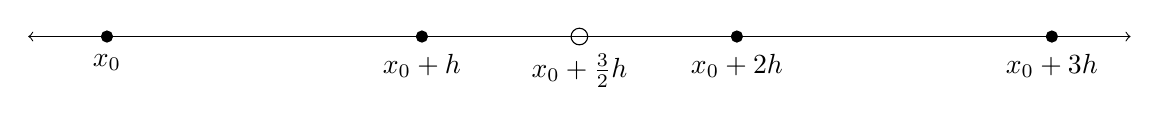
\begin{tikzpicture}
    \draw[<->] (-7,0) -- (7,0) node[below]{};
    \foreach \x/\label in {-6/\(x_0\), -2/\(x_0 + h\), 2/\(x_0 + 2h\), 6/\(x_0 + 3h\)} {
        \draw[fill] (\x, 0) circle (2pt);
        \node[below] at (\x,-0.1) {\label};
    }
    \draw (0, 0) circle (3pt);
    \node[below] at (0, -0.1) {\(x_0 + \frac{3}{2}h\)};
\end{tikzpicture}
\end{center}

using a direct method as discussed in Section 4.1.

\bigskip

We begin by finding the interpolating polynomial of least degree for this stencil. Using Lagrange's interpolation formula:
\[
    L(x_0 + \theta h) = \frac{(\theta - 1)(\theta - 2)(\theta - 3)}{(-1)(-2)(-3)}f(x_0) + \frac{\theta(\theta - 2)(\theta - 3)}{(1)(-1)(-2)}f(x_0 + h)
\]
\[
    + \frac{\theta(\theta - 1)(\theta - 3)}{(2)(1)(-1)}f(x_0 + 2h) + \frac{\theta(\theta - 1)(\theta - 2)}{(3)(2)(1)}f(x_0 + 3h)
\]
\[
    =-\frac{(\theta - 1)(\theta - 2)(\theta - 3)}{6}f(x_0) + \frac{\theta(\theta - 2)(\theta - 3)}{2}f(x_0 + h)
\]
\[
    - \frac{\theta(\theta - 1)(\theta - 3)}{2}f(x_0 + 2h) + \frac{\theta(\theta - 1)(\theta - 2)}{6}f(x_0 + 3h)
\]
We take the derivative twice with respect to \(\theta\) to get that
\[
    h^2L''(x_0 + \theta h) = \theta \left(\frac{f(x_0 + h)}{2} - \frac{f(x_0 + 2h)}{2} + \frac{f(x_0 + 3h)}{6}\right)
\]
\[
    + (\theta - 1)\left( -\frac{f(x_0)}{6} - \frac{f(x_0 + 2h)}{2} + \frac{f(x_0 + 3h)}{6} \right) 
\]
\end{question}

\begin{question}{4}
\textbf{(4.2, \#3c)} Over the same stencil as in the previous question, derive an approximation formula for the second derivative \( f'' \) but now using undetermined coefficients.
\end{question}

\begin{question}{5}
\textbf{(Based on 4.1, \#19)} Let \( x_0, x_0 + \alpha h, x_0 + 2h \) be nodes where \( \alpha \neq 0,2 \).

\begin{enumerate}[label=\alph*.]
    \item Write the first Taylor polynomials of \( f(x_0 +\alpha h) \) and \( f(x_0 +2h) \) around \( x = x_0 \), then use these to show that:
    \[
    f'(x_0) = \frac{1}{2h} \left[ \frac{-2+\alpha}{\alpha} f(x_0) + \frac{4}{\alpha(2-\alpha)} f(x_0 + \alpha h) - \frac{\alpha}{2-\alpha} f(x_0 + 2h) \right].
    \]

    \item Now show that the same result is obtained when using the method of undetermined coefficients.
\end{enumerate}
\end{question}

\begin{question}{6}
\textbf{(4.2, \#4i)} Use undetermined coefficients to derive an approximation formula for the integral over the stencil:

\begin{center}
\begin{tikzpicture}
    \draw[<->] (-1,0) -- (7,0);
    \draw[{Bracket[width=3mm]}-{Bracket[width=3mm]}] (0, 0) -- (6,0);
    \foreach \x/\label in {0/\(x_0\), 4/\(x_0 + \frac{4}{3}h\), 6/\(x_0 + 2h\)} {
        \draw[fill] (\x, 0) circle (2pt);
        \node[below] at (\x,-0.1) {\label};
    }

\end{tikzpicture}
\end{center}

\end{question}

\vfill
\centerline{End of Assignment 3}

\end{document}